%%%%%%%%%%%%%%%%%%%%%%%%%%%%
%%                        %%
%%   John L. Darcy's CV   %%
%%                        %%
%%%%%%%%%%%%%%%%%%%%%%%%%%%%
%
% Preamble:
  \documentclass{article} 
  \usepackage[margin=15mm]{geometry} % 15 mm margins all around
  \usepackage{hyperref} % for hyperlinks
  \usepackage{fontawesome} % for some symbols, needs: sudo apt-get install texlive-fonts-extra 
  \usepackage{multicol} % for multiple columns of text
  \usepackage{graphicx} % for pdf figures
  \usepackage{changepage} % for the adjustwidth environment
  \usepackage{enumitem} % makes bulleted lists
  \usepackage[utf8]{inputenc} % for utf8 characters like ʻokina
  \usepackage{float}    % used for figures
  \usepackage{caption}        % used for figures
  \usepackage{subcaption}     % used for figures
  \setlength\parindent{0pt} % no indentation allowed
  %
  \setlength{\multicolsep}{0pt}% remove vertical space for multiple columns
  \hypersetup{
    colorlinks   = true, %Colours links instead of ugly boxes
    urlcolor     = blue, %Colour for external hyperlinks
    linkcolor    = blue, %Colour of internal links
    citecolor    = black %Colour of citations
  }
  \usepackage[backend=biber, style=numeric-comp, maxbibnames=99, sorting=none, giveninits, terseinits]{biblatex} % note 'giveninits' replaces 'firstinits' for some stupid reason
  \renewbibmacro{in:}{} % removes "in:" before journal names
  \addbibresource{allrefs.bib}
  %
  % The following is a giant mess that makes the bibliography align with bulleted lists
  % (and gives each bib entry more room.... why was this so damn hard???)
  \defbibenvironment{bibliography}{
    \list{
      %% this is executed 
      \printfield[labelnumberwidth]{labelnumber}%
      \setlength{\labelwidth}{\labelnumberwidth}%
    }{
      \setlength{\leftmargin}{3mm}%
      \addtolength{\leftmargin}{\labelsep}%
      \setlength{\itemsep}{\bibitemsep}%
      \setlength{\parsep}{\bibparsep}%
    }
  }{\endlist}{\item}
  %
  % This should make my name bold in all the citations, AND remove commas
  % between last and first inits. "Darcy, JL" -> "Darcy JL"
  % by Zarko:
  % https://tex.stackexchange.com/questions/33330/make-one-authors-name-bold-every-time-it-shows-up-in-the-bibliography
  \usepackage{xstring}
  \usepackage{etoolbox}
  \newboolean{bold}
  \newcommand{\makeauthorsbold}[1]{%
    \DeclareNameFormat{author}{%
    \setboolean{bold}{false}%
      \renewcommand{\do}[1]{\expandafter\ifstrequal\expandafter{\namepartfamily}{####1}{\setboolean{bold}{true}}{}}%
      \docsvlist{#1}%
      \ifthenelse{\value{listcount}=1}
      {%
        {\expandafter\ifthenelse{\boolean{bold}}{\mkbibbold{\namepartfamily\addspace \namepartgiveni}}{\namepartfamily\addspace \namepartgiveni}}%
      }{\ifnumless{\value{listcount}}{\value{liststop}}
        {\expandafter\ifthenelse{\boolean{bold}}{\mkbibbold{\addspace \namepartfamily\addspace \namepartgiveni}}{\addspace \namepartfamily\addspace \namepartgiveni}}%
        {\expandafter\ifthenelse{\boolean{bold}}{\mkbibbold{\addspace \namepartfamily\addspace \namepartgiveni\isdot}}{\addspace \namepartfamily\addspace \namepartgiveni\isdot}}%
        }
      \ifthenelse{\value{listcount}<\value{liststop}}
      {\addcomma\space}{}
    }
  }
  \makeauthorsbold{Darcy}
  %
  % this puts my info at the bottom of the page next to the page number, so multiple sheets don't get mixed up
  \renewcommand{\thepage}{John L. Darcy~--~\arabic{page}}
  % this defines yen symbol as \yen : yen mark (taken from ascmac.sty for jlatex)
  \def\yen{{\setbox0=\hbox{Y}Y\kern-.97\wd0\vbox{\hrule height.1ex
  width.98\wd0\kern.33ex\hrule height.1ex width.98\wd0\kern.45ex}}}
  % actually begin document
  \begin{document}

%\centerline{\Huge\center\textbf{John L. Darcy, PhD}}
{\Huge \textbf{John L. Darcy, PhD}}
\hfill
\emph{Curriculum Vitae (\today)}
\vspace{1mm}
\hrule
\vspace{2mm}

\begin{adjustwidth}{5mm}{}
  \begin{multicols}{3}
    \faPhone \space +1 (303) 887 - 0477\\
    \faEnvelope \space \href{mailto:darcyj@colorado.edu}{darcyj@colorado.edu}\\
    \faGlobe \space \href{http://www.jldarcy.tk/}{jldarcy.com}\\
    \faGithub \space \href{https://github.com/darcyj}{github.com/darcyj}\\
    \faInstagram/\faTwitter \space \href{https://www.instagram.com/jld.adventures/}{@JohnLDarcy}\\
    \faMortarBoard \space \href{https://scholar.google.com/citations?user=z24F3PYAAAAJ}{Google Scholar link}
  \end{multicols}
\end{adjustwidth}

%
\vspace{2mm}
%
{\large\textbf{Research Emphasis}}
\begin{adjustwidth}{5mm}{}
  In my research, I use mathematical models to understand how microbial communities change over time and space. My research has spanned several different study systems, including the human microbiome, mouse microbiome, native Hawaiian plants, and soil microbes living in extreme environments across the world. My most recent work at CU Anschutz uses a mathematical model I developed to ask to what extent microbes are more likely to join a microbiome if they already have a close relative living there.
\end{adjustwidth}
%
\vspace{2mm} 
%
{\large  \textbf{Post-Doctoral Training}}
\begin{itemize}[noitemsep,topsep=0pt, leftmargin=5mm]
  \item US NIH NLM Computational Biology Post-Doctoral Fellowship at University of Colorado Anschutz Medical Campus, working with Catherine Lozupone. \mbox{Fall 2018 - present.}
  \item Post-doctoral researcher at University of Hawai'i at Mānoa, with Anthony Amend. \mbox{Fall 2017 - 2018.}
\end{itemize}
%
\vspace{2mm}
{\large  \textbf{Education}}
\begin{itemize}[noitemsep,topsep=0pt, leftmargin=5mm]
  \item PhD in Ecology and Evolutionary Biology from University of Colorado, Boulder (2017). Partly done at Duke University. Dissertation title: Biogeographic and biogeochemical drivers of microbial community assembly. Advised by Steve Schmidt (Boulder) and Diana Nemergut (Duke). 
  \item BA in Molecular, Cellular, and Developmental Biology (2010).
\end{itemize}
% first author citations - found in allrefs.bib tagged with keywords = {firstauthor}
\vspace{2mm}
{\large  \textbf{First-Author Publications}}\space\emph{(incl.\ equal contribution of first two authors)}
\vspace{-1em}\vspace{1mm}
\begingroup
	\setlength\bibitemsep{0pt}
	\nocite{*}
	\printbibliography[keyword=firstauthor, heading=none]
\endgroup
% coauthor citations - found in allrefs.bib tagged with keywords = {coauthor}
\vspace{-1em}\vspace{3mm}
{\large  \textbf{Co-Author Publications}}
\vspace{-1em}\vspace{1mm}
\begingroup
  \setlength\bibitemsep{0pt}
  \nocite{*}
  \printbibliography[keyword=coauthor, heading=none]
\endgroup
%
\vspace{0.5em}
%
{\large  \textbf{Publication Metrics}}
\begin{adjustwidth}{5mm}{}
  \begin{multicols}{2}
    \begin{itemize}[noitemsep,topsep=0pt, leftmargin=0mm]
      \item 48 published papers
      \item 1897 citations (as of 08/2021)
      \item h-index = 19
      \item i10-index = 26
    \end{itemize}
  \end{multicols}
\end{adjustwidth}
\vspace{3mm}
{\large  \textbf{Mentorship and Team Leadership}}
\begin{itemize}[noitemsep,topsep=0pt, leftmargin=5mm]
  \item Mentored Matthew Marshall, an undergraduate student as part of CU Anschutz Summer Bioinformatics Fellowship. I mentored Matt in developing a computer program that analyzes microbial communities in a competitive-lottery framework. We met twice weekly, and I created a production schedule and advised Matt on both programming and writing. Matt is preparing software for pulic release, and has written a release note for publication.
  \item Led a team at UH to develop and test a 3D-printed air sampler, to be used in large-scale sampling of air microbiota on the Hawaiian Islands. Team included 2 PhD students and 3 undergraduate students. Samplers were succesfully deployed in-situ and operated without supervision in the rainforest for multiple days until collected.
  \item Advised Adam Solon's honors thesis project in 2016. Adam used Illumina sequencing to compare microbial communities from multiple sites in the Chilean Atacama Desert, and this work is now published in Microbial Ecology \cite{Solon2018}. He was awarded summa cum laude.
  \item Advised Cerrise Weibern honors thesis project in 2015. She sequenced genomes of 8 Janthinobacterium strains and constructed a robust phylogeny of the species. She was awarded magna cum laude.
  \item Advised Zack Schubert's honors thesis project in 2014. I taught him how to implement complex simulation models in R, and together we made and compared mathematical models of water availability in soil undergoing freeze-thaw cycling. He was awarded summa cum laude.
  \item Mentored three undergraduate students from 2012 to 2014: Todd BT, Schrepel WA, and Choi RB. All three performed and helped design experiments. Todd BT is a co-author on several publications.
  \item Mentored two local middle school students, who completed a science fair project on E. coli transgenics. They won first prize in their school science fair competition, and went on to compete at state level.
\end{itemize}
\vspace{3mm}
{\large  \textbf{Teaching}}
\begin{itemize}[noitemsep,topsep=0pt, leftmargin=5mm]
  \item Started “Aloha R”, a computational biology workshop for graduate students at UH (Spring 2018). Weekly meetings focused on core programming skills, since many students view R as a “copy and paste” analytical platform rather than a robust programming environment. I also emphasized code documentation and repeatability.
  \item Guest lecturer for Ecology of Microbial Symbiosis (Spring 2018). Taught 2 lecture classes reviewing bioinformatics approaches used by microbial symbiosis researchers.
  \item Guest lecturer for Microbial Ecology (Fall 2016) Taught 3 lecture classes introducing students to modern molecular and bioinformatic approaches to microbial ecology.
  \item Ecology Lab TA (Fall 2013) Taught ecological theory and field methods, as well as basic statistics and computer programming in R. Three-hour periods with 20 students, 2x/week.
  \item Microbiology lab TA (Spring 2012) Taught basic microbiological technique, and modern molecular methods. Also wrote weekly quizzes and gave recitation. Two-hour periods with 18 students, 4x/week.
\end{itemize}
\vspace{3mm}
{\large  \textbf{Funding and Awards}}
\begin{itemize}[noitemsep,topsep=0pt, leftmargin=5mm]
  \item NIH NLM Computational Biology Postdoctoral Fellowship (present position).
  \item 2019 Front Range Microbiome Symposium award for best presentation. \$100.
  \item International Geological Society travel grant. Kyoto, Japan, December 2017. \yen100,000.
  \item Mycological Society of America travel award. San Juan, Puerto Rico, December 2017. \$2,500.
  \item SCAR XIIth International Biology Symposium Travel Grant. KU Leuven, December 2016. \$2,500.
  \item Remote (control) sensing: using a drone for environmental science. CU EBIO grant, April 2014. \$992.
  \item High-throughput climate change modeling from the gene’s perspective. Dean’s Graduate Student Research Grant Award, CU Boulder, October 2014. \$5,000.
\end{itemize}
%\vspace{3mm}
\pagebreak
{\large  \textbf{Selected Presentations and Posters}}
\begin{itemize}[noitemsep,topsep=0pt, leftmargin=5mm]
  \item Nepotism and Specificity In the human microbiome (Invited talk, 2020). CU Anschutz Computational Biology seminar series. Aurora, Colorado.
  \item What are compositional data and why do I care? (Invited talk, 2020). CU Anschutz Computational Biology seminar series. Aurora, Colorado.
  \item A phylogenetic model for the arrival of species into microbial communities (Invited talk, 2019). NIH NLM Computational Biology Training Conference. Indianapolis, Indiana.
  \item Specificity analysis of microbiome data: All the math (Chalk talk, 2019). CU Anschutz Microbiome group chalk talk.
  \item Monte Carlo analysis of Foliar Fungal Endophytes reveals habitat specificity to elevation, precipitation, and host plants (Seminar, 2019). Hawaii Ecosystems Conferencein  Hilo, Hawaii.
  \item A phylogenetic model for the arrival of species into microbial communities (Poster, 2019). Front Range Microbiome Symposium in Fort Collins, Colorado.
  \item Cryoconite holes are microbial islands (Seminar, 2018). International Glaciological Society meeting in Kyoto, Japan.
  \item Island biogeography of glacial microbiota in Antarctica’s Taylor Valley and around the world (Seminar, 2017). Scientific Committee on Antarctic Research Biology meeting in Leuven, Belgium.
  \item Using Adobe Illustrator to make scienetific figures (Seminar, 2016). CU Boulder EBIO dept. Brown-bag talk.
  \item Phylogenetic and biogeochemical characterization of a debris-covered glacier (Poster, 2013). ASM General Meeting 2013 in Denver CO.
  \item Identification and characterization of microbial communities in high-elevation snowpacks (Poster, 2013). LTER meeting 2013 in Estes Park, CO.
  \item Comparing spatial distributions of microorganisms using minimal genetic distance. ASM General Meeting 2012 in San Francisco, CA.
\end{itemize}
\vspace{3mm}
{\large  \textbf{Peer-Review}}\\
Journals I've peer-reviewed for are listed on my \href{https://publons.com/researcher/1262170/john-l-darcy/peer-review/}{Publons} profile (slow to update). 
\\\begin{tabular}{l l l}
  Journal & Number of Reviews & Recency\\
  \hline
  NPJ Biofilms and Microbiomes & 2 & 2020\\
  Nature Communications & 3 & 2019\\
  Ecology and Evolution & 1 & 2020\\
  Data in Brief & 1 & 2020\\
  PeerJ & 1 & 2019\\
  Plant and Soil & 1 & 2019\\
  Molecular Ecology & 4 & 2018\\
  Environmental Microbiology & 1 & 2018\\
  Frontiers in Microbiology & 1 & 2017\\
  The ISME Journal & 1 & 2018\\
  Journal of Biogeography & 1 & 2018\\
\end{tabular}
\vspace{3mm}

{\large  \textbf{Data and Analytical Skillset}}
  \begin{adjustwidth}{2mm}{}\begin{multicols}{2}
    % column 1:
    Spatial analyisis \cite{Darcy2018a,Darcy2011a,Darcy640029}\\
    Spatiotemporal analysis \cite{Darcy640029,Darcy2017,Nemergut2016}\\
    Comparative genomics \cite{Darcy2018,Lynch2014}\\
    Mathematical modeling and simulation modeling \cite{Darcy685644,Darcy640029, Darcy2016}\\
    Geographic information systems (GIS) \cite{Darcy640029,Darcy2018a,Darcy2017}\\
    Meta-analysis \cite{Darcy685644,Darcy2018a,Darcy2011a}\\
    Project-level version control \cite[\href{https://github.com/darcyj/specificity}{specificity} R package]{Darcy2018}\\
    High-throughput sequencing analysis \cite{Darcy685644,Darcy640029,Darcy2018a}\\

    % column 2:
    Temporal analysis \cite{Darcy685644,Knelman2014,Kennedy2016}\\
    Landscape ecology \cite{Darcy640029,Darcy2018,Darcy2017}\\
    Phylogenetics \cite{Darcy2011a,Schmidt2015a,Naff2013}\\
    Multivariate satistical analysis \cite{Darcy640029,Darcy2017,Gendron2019}\\
    Spatial experimental design \cite{Darcy2018a,Darcy2017,Darcy2018}\\
    Machine learning (current project)\\
    Genome assembly and metagenome assembly \cite{Darcy2018,Lynch2014}\\
    High-throughput sequencing pipelining \cite{Darcy685644,Darcy640029,Darcy2018a}

  \end{multicols}\end{adjustwidth}

{\large  \textbf{Programming Languages}}
\\\begin{tabular}{l l l}
  Language & Proficiency & Example\\
  \hline
  R & (expert) & \href{https://github.com/darcyj/specificity}{github.com/darcyj/specificity}\\
  Shell/Bash & (advanced) & \href{https://github.com/darcyj/pd_assemb}{github.com/darcyj/pd\_assemb}\\
  C++ & (intermediate) & \href{https://github.com/darcyj/specificity}{github.com/darcyj/specificity}\\ 
  Python & (intermediate) & \href{https://github.com/darcyj/cardpricer}{github.com/darcyj/cardpricer}\\
  \LaTeX & (beginner) & \href{https://github.com/darcyj/cv}{github.com/darcyj/cv}\\
  HTML+CSS & (beginner) & \href{jldarcy.tk}{jldarcy.tk}\\
\end{tabular}

%\vspace{3mm}
\pagebreak
{\large  \textbf{General Software Knowledge}}
  \begin{adjustwidth}{2mm}{}\begin{multicols}{3}
    % column 1:
    Linux system admininstration\\
    Slurm\\
    qGIS\\
    Rstudio\\
    Mendeley\\
    % column 2:
    Microsoft Office (Word, Excel, Ppt)\\
    Libre Office (Writer, Calc)\\
    Sublime Text\\
    MonoDevelop\\
    High performance computing (HPC)\\
    % column 3:
    Adobe Illustrator\\
    Adobe Photoshop\\
    Zoom\\
    Unix command line tools
  \end{multicols}\end{adjustwidth}

\vspace{3mm}
{\large  \textbf{Molecular Biology and Bioinformatics Software Knlowledge}}
  \begin{adjustwidth}{2mm}{}\begin{multicols}{3}
    % column 1: (microbiome stuff)
    Qiime/Qiime2\\
    Phyloseq\\
    Usearch/Vsearch\\
    DADA2\\
    BLAST\\
    SRA Toolkit\\
    % column 2: (genome assembly stuff)
    SOAPdenovo\\
    MetaVelvet\\
    MaxBin\\
    metaSPAdes\\
    Samtools\\
    BWA\\
    % column 3: (phylogenetics stuff)
    MrBayes\\
    FastTree\\
    MUSCLE\\
    SEPP\\
    ITSxpress\\
    Fastx Toolkit
  \end{multicols}\end{adjustwidth}

\vspace{3mm}
{\large  \textbf{Laboratory Skillset}}
  \begin{adjustwidth}{2mm}{}\begin{multicols}{3}
    % column 1: (microbiology stuff)
    Bacterial culture\\
    Microcosm experiments\\
    Media prep/creation\\
    Culture preservation\\
    Cloning\\
    PCR/qPCR/Colony PCR\\
    % column 2: (high throughput sequencing stuff)
    Illumina sequencing prep\\
    Sanger sequencing prep\\
    DNA/RNA purification\\
    Qubit/Nanodrop\\
    Gel electrophoresis\\
    Plate reader analyses\\
    % column 3: (microscopy stuff)
    Fluorescence microscopy\\
    Phase-contrast microscopy\\
    Staining/fixing\\
    Computational microscopy\\
    Primer development\\
    Various soil analyses
  \end{multicols}\end{adjustwidth}

\vspace{3mm}
{\large  \textbf{Fieldwork Expertise}}
\begin{itemize}[noitemsep,topsep=0pt, leftmargin=5mm]
  \item Sample collection in extreme conditions at high altitude (\textgreater6000 masl).
  \item Drone flight and data capture at high altitude (\textgreater5000 masl).
  \item Sampling based off of remote sensing data and planned spatial experimental designs.
  \item Wilderness survival after a grizzly bear destroyed my tent+bag+pad followed by 12 hours of rain.
  \item Extemporaneous experimental design under hypoxic conditions.
  \item Logistic coordination with indigenous peoples in the Peruvian Andes.
  \item Extended backpacking campaigns above 5000 masl.
  \item Experience in Antarctica’s McMurdo Dry Valleys, including helicopter travel, ice climbing, and glacier traverse.
  \item Rainforest backpacking and sample collection in Hawaii.

\end{itemize}

\vspace{3mm}
\captionsetup[figure]{labelformat=empty} % gets rid of "Figure 1" in captions
{\large  \textbf{Photos}}
\begin{figure}[H]
  \begin{minipage}{0.47\textwidth}
    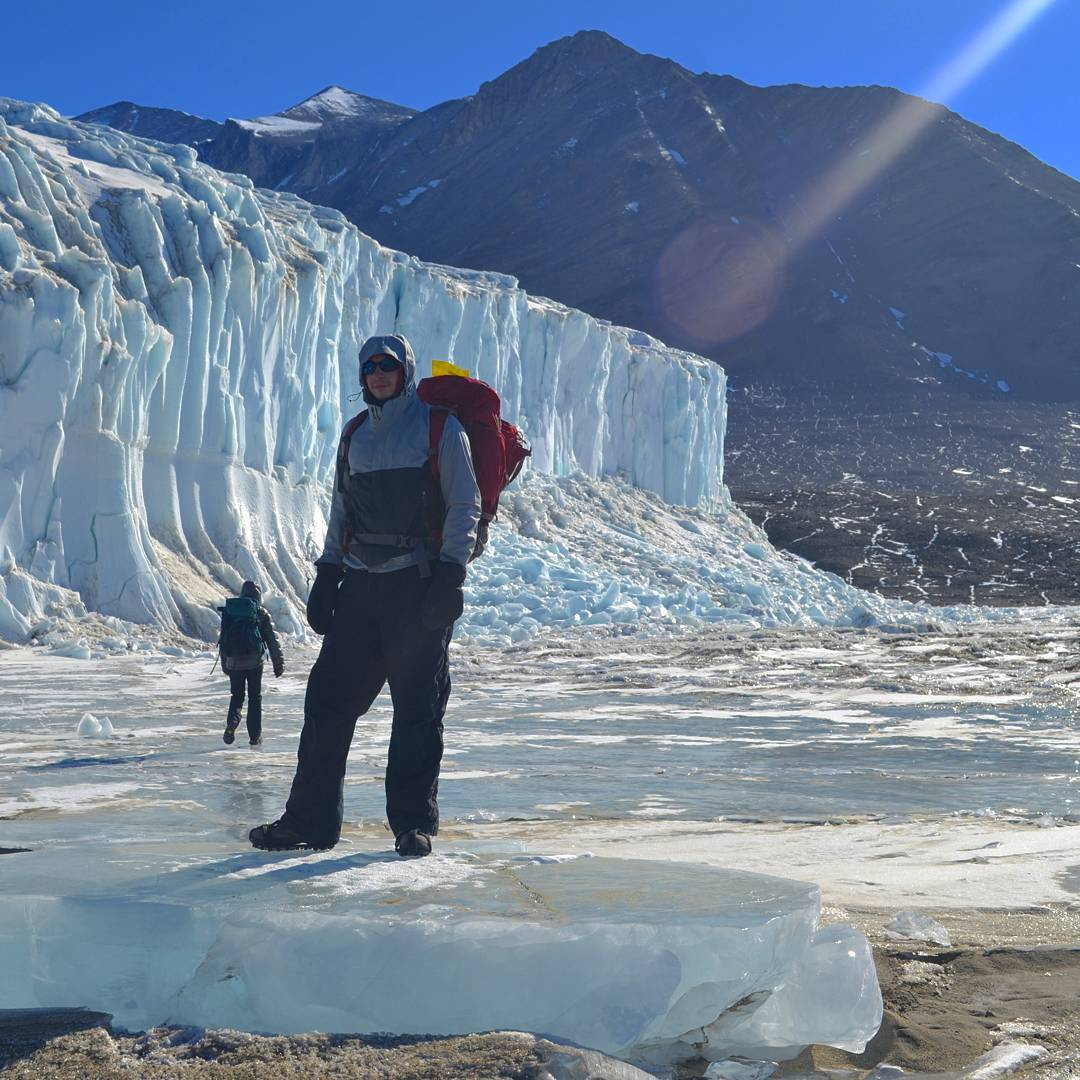
\includegraphics[width=\linewidth]{pix/at_canada_term_2016.jpg}
    \caption{Standing at the terminus of the Canada Glacier in the McMurdo Dry Valleys, Antarctica.}
    \end{minipage}
  \hspace{\fill} % note: no blank line here
  \begin{minipage}{0.47\textwidth}
    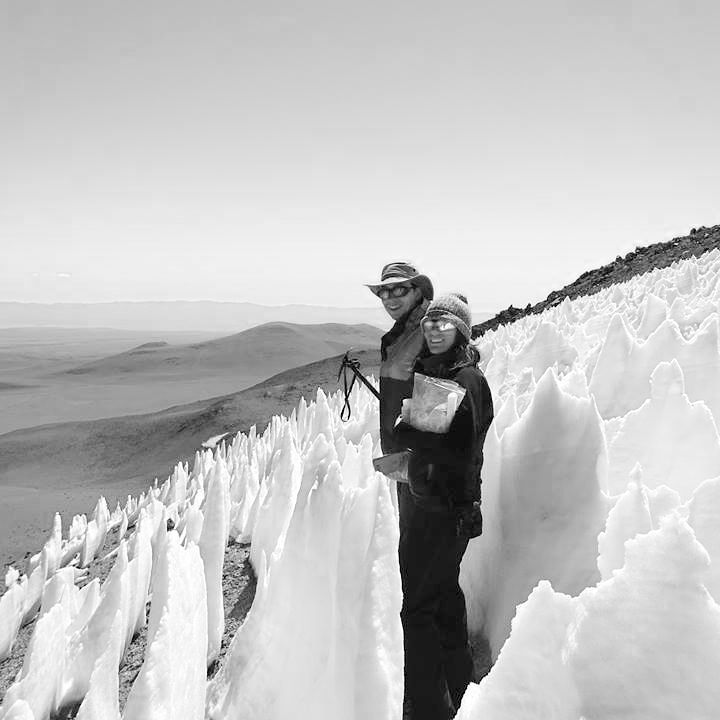
\includegraphics[width=\linewidth]{pix/penitentes_2016.jpg}
    \caption{With my labmate Lara amongst penitentes on the stratovolcano Llullaillaco in the Chilean Andes.}
    \end{minipage}
\end{figure}




\end{document}